\section{Evaluation}\label{Evaluation}

In diesem Kapitel wollen wir uns jetzt mit der Analyse der einzelnen 
Optimierungsmethoden beschäftigen. Mithilfe des vorherigen Kapitel wollen
wir nachweisen, dass ein theoretisch besserer Algorithmus auch wirklich besser 
arbeitet. Was in diesem Fall ``besser'' bedeutet soll ebenfalls geklärt werden.

\subsection{Test Datensatz} \label{Test Datensatz}

Um ein neuronales Netz zu bewerten, brauchen wir zunächst einige Test Daten,
hierbei werden die beiden frei verfügbaren Datensätze, der \textit{Boston House Price}
Datensatz und der \textit{Breast Cancer} Datensatz, benutzt. Beide sind im \textit{scikit-learn}
Paket \cite{scikit-learn} enthalten. 

\subsubsection{Boston House Price} \label{Boston House Price}

Der \textit{Boston House Price} Datensatz besteht aus einem Regressionsproblem.
Das bedeutet, dass wir eine reelle Zahl mit unserem Netz voraussagen wollen, nämlich den
Preis eines Hauses in Boston. Damit das das  Netz lernen kann gibt es einige 
explanatorische Variablen wie unter anderem

\begin{itemize}
    \item \textbf{CRIM}: Die Verbrechensrate pro Kopf.
    \item \textbf{RM}: Die Anzahl der Räume im Haus.
    \item \textbf{TAX}: Steuer die auf das Grundstück gezahlt werden muss.
    \item \textbf{DIS}: gewichteter Abstand zum Zentrum von Boston. 
\end{itemize}

Mit diesen, insgesamt 13 Hilfsvariablen soll das Netz den Haus Preis voraussagen.

\begin{figure}[htbp] 
    \centering
       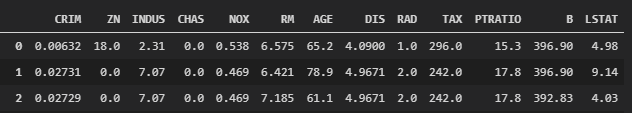
\includegraphics[width=1.0\textwidth]{abb/BostonBeispiel.PNG}
    \caption{Beispiel des Boston Datensatzes}
    \label{fig:BostonBeispiel}
\end{figure}


\subsubsection{Breast Cancer} \label{Breast Cancer}

Der \textit{Breast Cancer} Datensatz hingegen besteht aus einem binären Klassifikationsproblem.
Das bedeutet, dass das Netz nur ``ja'' oder ``nein'' kodiert als eins oder null, voraussagen
soll. Hierbei bedeutet ein Ja, dass diese Person Brustkrebs hat. Hier gibt es 
wieder einige explanatorische Variablen, die dem Netz helfen sollen zu lernen.
Diese sind Eigenschaften des Nukleus einer entommenen Brustzelle


\begin{itemize}
    \item \textbf{radius}: Radius des Nukleus
    \item \textbf{texture}: Standardabweichung der Graustufenwerte
    \item \textbf{symmetry}: Symmetrie des Nukleus
    \item \textbf{smoothness}: Lokale Abweichung der Radius Länge
\end{itemize}

Insgesamt besteht der Datensatz aus 30 solchen Variablen.

\begin{figure}[htbp] 
    \centering
       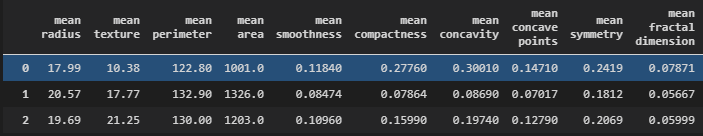
\includegraphics[width=1.0\textwidth]{abb/BreastCancerBeispiel.PNG}
    \caption{Beispiel des Breast Caner Datensatzes}
    \label{fig:BreastCancerBeispiel}
\end{figure}

\subsection{Metrik} \label{Metrik}

Bevor wir mit dem Vergleich der verschiedenen Optimierungsmethoden der Gradienten
beginnen können, brauchen wir ein Maß für die Güte eines Ergebnisses. 
Dafür müssen wir eine Metrik definieren. Sinnvoll ist es ein neuronales Netz
daran zu messen, wieviel es richtig bewertet hat. Richtig ist im Falle des \textit{Breast Cancer}
Datensatzes einfach ob das Netz ja zu ja und nein zu nein gesagt hat. Im Falle 
des \textit{Boston House Price} Datensatzes ist richtig, wenn der Abstand vom
vorhergesagten zum echten Preis möglichst klein ist. Dies gibt uns eine 
Vielzahl von Metriken die diese Voraussetzungen erfüllen.\\

Günstiger Weise benötigen wir bereits durch das Training des neuronalen Netzes 
eine Gütefunktion die angibt ob sich die Parameter in die richtige Richtung bewegen.
Diese ist die in Abschnitt \ref{Neuronale Netze} bereits besprochene Fehlerfunktion des 
Netzes. Diese sollte unsere erste Form einer Metrik sein um das Neuronale Netz zu bewerten.

Für den \textit{Boston House Price} Datensatz ist diese Fehlerfunktion die
\textit{mittlere quadratische Abweichung}.

\begin{definition}
    \cite[S.344]{Fahrmeir.2016} Die \textbf{mittlere quadratische Abweichung} für eine Stichprobe $x_1,...,x_n$
    mit Schätzwerten $\hat{x}_1,...,\hat{x}_n$ ist definiert durch
    \begin{align}
        \frac{1}{n}\sum\limits_{i=1}^{n} (\hat{x}_i-x_i)^2
    \end{align}
\end{definition}

Dies ist die typische Fehlerfunktion für Regressionsprobleme. Man mag sich fragen
warum diese quadriert wird und nicht der absolute Abstand zum echten Wert genommen
wird, wie vorher überlegt. Diese Funktion ist aber diejenige aus der wir den Gradienten
berechnen wollen, also muss sie differenzierbar sein, was das Quadrat gewährleistet.\\

Für den \textit{Breast Cancer} Datensatz ist diese Funktion jedoch unzureichend, da 
nur null oder eins im Wertebereich der mittleren quadratischen Abweichung vorkommen würden.
Da es sich hier um ein binäres Klassifikationsproblem handelt, eignet sich die \textit{binäre Kreuzentropie}.

\begin{definition}
    \cite{Rubinstein.2004} Die \textbf{binäre Kreuzentropie} für eine Stichprobe $x_1,...,x_n$
    mit Schätzwerten $\hat{x}_1,...,\hat{x}_n$ ist definiert durch
    \begin{align}
        \frac{1}{n}\sum\limits_{i=1}^{n} x_i log(\hat{x}_i) + (1-x_i)log(1-\hat{x}_i)
    \end{align}
    wobei $log$ der natürliche Logarithmus ist.
\end{definition}

Diese Fehlerfunktion ist geeignet für Wertebereiche zwischen null und eins. Also genau 
passend für ein zwei Klassen Klassifikationsproblem. \\

Diese beiden Fehlerfunktionen geben uns eine erste Idee für die Güte des neuronalen 
Netzes und deren Prädiktion und damit auch einen Indikator, welches
Netz den besseren Optimierungsalgorithmus besitzt, wenn sonst alle Parameter 
gleich bleiben. 
Zusätzlich nehmen wir um mehr Vergleichbarkeit zu schaffen eine weitere Fehlerfunktion hinzu,
die nur der Evaluierung der besseren Optimierungsmethode dient und nicht 
für das Gradienten Abstiegsverfahren genutzt wird.
Im Falle des \textit{Boston House Price} Datensatzes benutzen wir noch den 
\textit{Mittleren absoluten Fehler}.

\begin{definition}
    Der \textbf{Mittlere absolute Fehler} für eine Stichprobe $x_1,...,x_n$
    mit Schätzwerten $\hat{x}_1,...,\hat{x}_n$ ist definiert durch
    \begin{align}
        \frac{1}{n}\sum\limits_{i=1}^{n} | \hat{x}_i-x_i |
    \end{align}
\end{definition}

Dies ist die intuitivere Definition des Fehlers und ist somit geeignet um die
Optimierungsmethoden zu vergleichen.

Für den \textit{Breast Cancer} Datensatz benutzen wir zusätzlich die \textit{Accuracy},
um die Ergebnisse des neuronalen Netzes vergleichbarer zu machen.

\begin{definition}
    Die \textbf{Accuracy} einer Stichprobe der Größe $n$ ist definiert durch 
    \begin{align}
        Accuracy = \frac{\text{Anzahl korrekter Voraussagen}}{n}
    \end{align}
\end{definition}

Diese ist ebenfalls das intuitivere Verständnis der Güte eines neuronalen Netzes und hilft
somit bei der Auswertung der Optimierungsalgorithmen.

\subsection{Programm} \label{Programm}
 
Für einen Aufbau eines solchen Netzes und die Anwendung des Gradienten Abstiegsverfahrens
gibt es bereits verschiedenste Frameworks. Diese stehen vor Allem in \textit{Python} zur
Verfügung, da diese eine der vorrangigen KI Sprachen ist. Aus diesem Grund 
wird das folgende Programm für die Auswertung der Optimierungsalgorithmen, auf unseren
zwei Test Datensätzen, ebenfalls in \textit{Python} implementiert sein. 

\subsubsection{Frameworks}

Um uns die Arbeit zu erleichtern und um die Optimierungsalgorithmen, sowie das 
neuronale Netz nicht selbst implementieren zu müssen benutzen wir einige Frameworks.

\begin{itemize}
    \item \textbf{Keras} \cite{chollet2015keras}: Ein Framework, um neuronale Netze durch ein ``Baustein'' artiges 
        Prinzip aufzubauen. 
    \item \textbf{Scikit-learn} \cite{scikit-learn}: Ein Framework, welches viele machine learning-
        sowie Vorverarbeitungsalgorithmen als Funktionsaufruf zur Verfügung stellt.
    \item \textbf{Pandas} \cite{mckinney-proc-scipy-2010}: Ein Framework, was uns 
        tabellenartige Datenstrukturen zur Verfügung stellt, welche die Weiterverarbeitung vereinfachen.
    \item \textbf{Numpy} \cite{numpy}: Ein Framework für wissenschaftliche Berechnungen 
        in Python, wie zum Beispiel Matrizenmultiplikation.  
\end{itemize}

\subsubsection{Aufbau} \label{Aufbau}

Die Idee hinter dem Aufbau des Python Programms war eine Objekt orientierte Klassenlandschaft
zu erstellen, um möglichst allgemein die verschiedenen Optimierungsalgorithmen an unterschiedlichen 
Neuronalen Netzen und Datensätzen zu testen. Das folgende UML-Diagramm veranschaulicht
diese Prämisse.

\begin{figure}[htbp] 
    \centering
       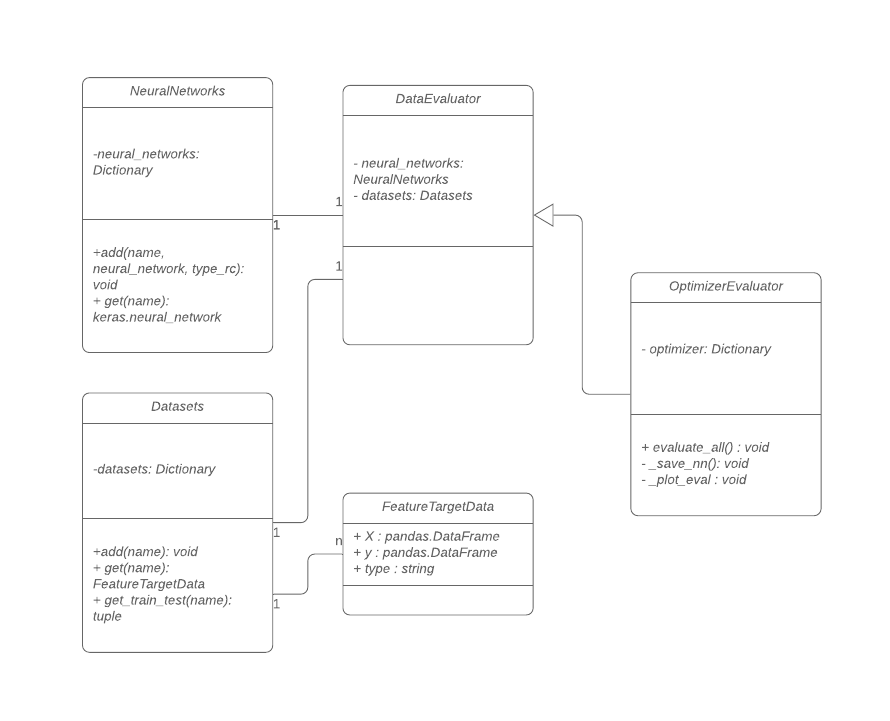
\includegraphics[width=1.0\textwidth]{abb/STI_fertig.png}
    \caption{UML-Diagramm des Python Programms}
    \label{fig:UML}
\end{figure}

Die wichtigste Klasse hier ist der \texttt{DataEvaluator}. Er verallgemeinert 
das Konzept einer Testklasse, die Neuronale Netze zu bestimmten Datensätzen auswertet.
Was dabei ausgewertet wird, wird allgemein gehalten. Die konkrete Implementierung erfolgt 
in der \texttt{OptimizerEvaluator} Klasse, die mit der \texttt{evaluate\_all} Methode
die eigentliche Auswertung der Optimierungsalgorithmen übernimmt. Diese 
erbt von \texttt{DataEvaluator} und besitzt somit dessen Attribute, die vom Typ
\texttt{NeuralNetworks} und \texttt{Datasets} sind.

Diese besitzen jeweils ein dictionary
Attribut, in dem sie nach dem key value Prinzip ihre jeweiligen Inhalte speichern.
In \texttt{Datasets} werden die Auszuwertenden Datensätze gespeichert. Diese Datensätze
sind vom Typ \texttt{FeatureTargetData}. 

Dieser neue Datentyp wird benötigt
um später einfach zwischen explanatorischen Variablen und Zielvariablen zu unterscheiden.
In \texttt{X} werden die explanatorischen Variablen gespeichert und in \texttt{y} die Zielvariable.
Zusätzlich speichern wir die Art der Vorhersage, die auf dem Datensatz möglich ist.
Also entweder ``Regression'' oder ``Klassifikation''. Wir benötigen diese Information, 
um später die richtigen Metriken auszuwählen. Wie in Abschnitt \ref{Metrik} erläutert, 
benutzen wir verschiedene Metriken für Regressions- und Klassifikationsprobleme.

In der \texttt{Neural Networks} Klasse werden die neuronalen Netze, die 
uns das Keras Framework zur Verfügung stellt gespeichert. Dabei wird nur deren
Struktur gespeichert. Die Gewichte werden erst später angepasst, wenn wir das Netz
auf einen Datensatz trainieren. 

\subsubsection{Netzstruktur}

Oftmals steht und fällt ein neuronales Netz mit seiner vorher festgelegten
Struktur. Diese kann das Netz nicht selbst lernen, sondern muss vom Menschen 
vorgegeben werden. Da unser Hauptfokus jedoch der Vergleich der Optimierungsalgorithmen
ist, und nicht der Aufbau eines perfekten neuronalen Netzes,
ist die Netzstruktur eher zweitrangig. Zusätzlich sind die 
Testdatensätze eher einfachere Probleme, die auch simple 
neuronale Netzstrukturen gut lernen können. Wichtig ist nur, dass wir immer 
den gleichen Netzaufbau für jede Optimierung benutzen um Vergleichbarkeit zu schaffen. 

Im folgenden soll die Netzstruktur, die wir für die Regressionsprobleme
des \textit{Boston House Price} Datensatzes benutzen erläutert werden.

\begin{lstlisting}[language=Python]
_regression_NN_boston = Sequential()
_regression_NN_boston.add(
    Dense(units=160, activation='relu', input_shape=(13,)))
_regression_NN_boston.add(Dense(units=64, activation='relu'))
_regression_NN_boston.add(Dense(units=1, activation='linear'))
\end{lstlisting}

Diese Definition ist für das \textit{Keras} Framework gedacht.
Hier definiert man jede Ebene des Netzes nacheinander. 
Wir initialisieren das Netz mit dem \texttt{Sequential} Konstruktor.
Das bedeutet, dass wir ein normales feed forward Netz bauen wollen,
wie in Abschnitt \ref{Neuronale Netze} erläutert. 
Nun fügen wir die erste Ebene des Netzes hinzu. Diese ist \texttt{Dense}, 
was bedeutet, dass jedes Neuron mit jedem verknüpft ist.
Außerdem sind insgesamt 160 Neuronen in dieser Ebene. 
Die Anzahl der Neuronen ist üblicherweise ein Indikator dafür, wie komplex das 
Netz ist und vor Allem wie komplex das Problem ist, welches das Netz versucht
zu lösen. Für diese einfache Problematik sollten 160 Neuronen jedoch ausreichen
\\

In dieser Ebene verwenden wir die nichtlineare Aktivierungsfunktion \textit{Relu},
wie in Definition \ref{Def:formales Neuron} bereits erläutert, wird diese nichtlineare
Funktion benötigt um nichtlineare Probleme zu lösen und macht somit das 
Gradienten Abstiegsverfahren erst notwendig.
Da es sich hier um eine innere Schicht eines feed forward Netzes handelt ist die
Wahl von Relu eindeutig. Diese hat sich in den letzen Jahren als beste 
Aktivierungsfunktion für innere Schichten herausgestellt. \cite[S. 226]{Goodfellow.2016}
Der Parameter \texttt{input\_shape} gibt an wie viele explanatorische Variablen
dem Netz zugeführt werden. Wie in Abschnitt \ref{Boston House Price} besprochen,
besitzt der \textit{Boston House Price} Datensatz 13 explanatorische Variablen.
Mit diesem Prinzip wird noch eine innere Schicht hinzugefügt und schließlich 
die Ausgabeschicht die nur aus einem einzigen Neuron besteht, da wir hier die
Zahl für den Preis erwarten.\\

Für den \textit{Breast Cancer} Datensatz ergibt sich ein ähnlicher Aufbau.

\begin{lstlisting}[language=Python]
_classification_NN_breast_cancer = Sequential()
_classification_NN_breast_cancer.add(
    Dense(40, input_shape=(30,), activation='relu'))
_classification_NN_breast_cancer.add(Dense(20, activation='relu'))
_classification_NN_breast_cancer.add(Dense(1, activation='sigmoid'))
\end{lstlisting}

Nur das hier in der Ausgabeschicht die \textit{Sigmoid} Funktion verwendet wird, 
da wir eine Zahl zwischen null und eins erwarten. Nämlich die Wahrscheinlichkeit
für Brustkrebs. 

\subsection{Auswertung} \label{Auswertung}

Nun ist alles bereit um die verschiedenen Netze mit unterschiedlichen Optimierungsalgorithmen
zu trainieren und diese anschließend mit den Metriken aus Abschnitt \ref{Metrik}
zu bewerten. 

\subsubsection{Erwartungen} \label{Erwartungen}

Wir werden die drei vorgestellten Algorithmen 
\begin{itemize}
    \item Stochastic Gradient Descent
    \item Adagrad
    \item ADAM
\end{itemize}

anwenden und ihre Performance mithilfe der Metriken messen. Der \textit{Stoachstic Gradient Descent}
ist dabei der simpelste Algorithmus. Also würden wir erwarten, dass dieser die schlechtesten 
Ergebnisse liefert. \textit{Adagrad} und \textit{ADAM} sind ähnlich, jedoch 
benutzt ADAM noch mehr Informationen als Adagrad. \textit{ADAM} sollte somit 
die beste Performance haben. Adagrad sollte aber auch nicht schlecht sein, da 
beide Datensätze eher klein sind und somit eine adaptive Anpassung der Gewichte
wichtig ist.

\subsubsection{Boston House Price Auswertung} \label{Boston House Price Auswertung}

Für die Auswertung des \textit{Boston House Price} Datensatzes haben wir den \textit{MSE} (in der Abbildung \ref{fig:BHPAuswertung} unter Loss) und den \textit{MAE} 
als Metrik ausgewählt. Umso niedriger diese Werte sind, desto besser hat das Netz den Hauspreis 
vorausgesagt. 

\begin{figure}[htbp] 
    \centering
       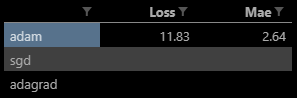
\includegraphics[width=0.6\textwidth]{abb/boston_score.png}
    \caption{Boston House Price Auswertung}
    \label{fig:BHPAuswertung}
\end{figure}

In Abbildung \ref{fig:BHPAuswertung} ist klar zu erkennen das keine Werte unter 
den beiden Optimierungsmethoden \textit{SGD} und \textit{Adagrad} eingetragen wurden.
Das liegt daran dass diese Optimierungsalgorithmen nicht konvergiert sind. 

\begin{figure}[htbp] 
    \centering
       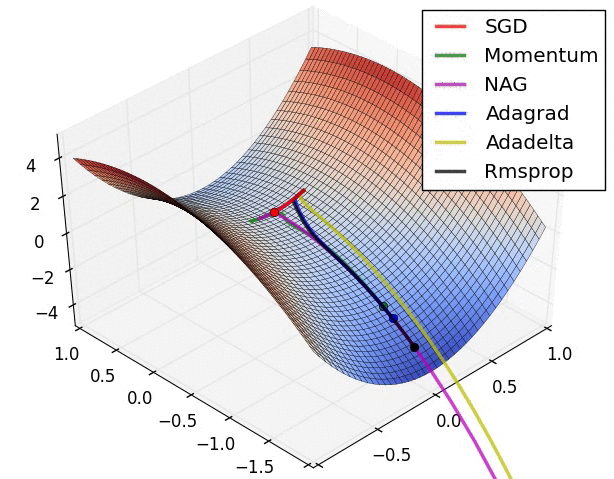
\includegraphics[width=0.6\textwidth]{abb/VisualizationDivergenz.PNG}
    \caption{Visualisierung Divergenz - Quelle: \url{https://imgur.com/a/Hqolp}}
    \label{fig:Divergenz}
\end{figure}

In Abbildung \ref{fig:Divergenz} sehen wir die Oberfläche für ein solches Ergebnis.
Die Algorithmen starten offensichtlich in der Nähe eines Sattelpunkts und folgen einem
unendlichen Abstieg. Bei \textit{ADAM} passiert dies jedoch nicht. Dieser ist offensichtlich
wesentlich robuster gegenüber solchen Sattelpunkten. 
Ein anderer Grund für eine solche Divergenz könnte beim Stochastic Gradient Descent auch eine 
unpassende Lernrate $\eta$ sein. Oft können solche Divergenzen auch durch eine schlechte 
Parametrisierung des Lernraums entstehen. Dadurch, dass die Distanzen in einem 13 dimensionalen 
Raum sehr groß werden, können solche Divergenzen begünstigt werden. 
Die Variablen wurden jedoch vor dem Training normalisiert, weswegen dieser Grund ausgeschlossen
werden kann. 

\subsubsection{Breast Cancer Auswertung} \label{Breast Cancer Auswertung}

Für die Auswertung des \textit{Breast Cancer} Datensatzes benutzen wir die Metriken 
der \textit{binären Kreuzentropie} (in Abbildungen \ref{fig:BCAuswertung} als Loss benannt)
und die Accuracy. Die binäre Kreuzentropie soll dabei möglichst klein sein, wogegen die Accuracy
möglichst nah bei eins sein sollte, um ein besseres Ergebnis zu liefern.  

\begin{figure}[htbp] 
    \centering
       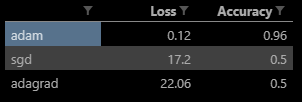
\includegraphics[width=0.6\textwidth]{abb/breast_cancer_score.PNG}
    \caption{Breast Cancer Auswertung}
    \label{fig:BCAuswertung}
\end{figure}

Hier sehen wir ebenfalls, dass \textit{ADAM} die besten Ergebnisse zeigt. 
Die beiden anderen Optimierungsalgorithmen zeigen deutlich stärkere Fluktuationen auf.
Interessant ist hier, dass der \textit{Stochastic Gradient Descent} besser performt als \textit{Adagrad}.
Dies liegt wahrscheinlich an der wie in Abschnitt \ref{Adagrad} besprochenen Summierung der Gradienten,
welche \textit{Adagrad} irgendwann stoppen lässt ein Minimum zu suchen.


\subsubsection{Vergleich mit der Literatur} \label{Vergleich mit Literatur}

In der Literatur ist ebenfalls oft die Rede von \textit{ADAM} als go-to Optimierungsalgorithmus,
da er sehr robust ist und man kein Parametertuning benötigt um gut Ergebnisse zu bekommen. 
\textit{Adagrad} hat offensichtlich Probleme mit Konvergenz, wie wir ebenfalls nachweisen konnte und ist 
daher nur in seltenen Fällen benutzbar, da die adaptive Anpassung der Parameter ebenfalls 
von \textit{ADAM} besser durchgeführt wird. Jedoch scheint der \textit{Stochastic Gradient Descent}
ebenfalls sehr wirkungsvoll zu sein. Das Problem ist jedoch, dass der \textit{Stochastic Gradient Descent}
eine gute Lernrate braucht, die nicht offensichtlich ist, wie wir in der Auswertung gesehen haben.
Außerdem braucht man eine gute Initialisierung und der Algorithmus braucht deutlich länger.
\cite[Abschnitt 4.10]{Ruder.9152016}